\paragraph{1. Library toevoegen}
Eerst moeten de libraries aan de root van ons project worden toegevoegd. 
Deze worden toegevoegd met volgende commando's:
\begin{minted}{bash}
npm install --save react-native-track-player
npm install --save react-native-video
\end{minted}

\paragraph{2. Package teruggeven}
Normaal gezien moet de package dan worden toegevoegd aan het 
\textit{android/app/src/} \textit{main/java/com/project/MainApplication.java} bestand.
Maar dit is niet meer nodig bij React Native 0.60+.

\paragraph{3. Audio library initialiseren}
Om de audio speler te kunnen gebruiken, moet een service bestand worden geregistreerd in de main 
component van de applicatie, meestal is dit het \textit{index.js} bestand.
\begin{minted}{javascript}
import TrackPlayer from 'react-native-track-player';
// AppRegistry.registerComponent(...);
TrackPlayer.registerPlaybackService(() => require('./service.js'));
\end{minted}
Daarna moet er een service worden aangemaakt in een apart \textit{service.js} bestand.
\begin{minted}{javascript}
module.exports = async function() {
    // ...
}
\end{minted}
Tot slot moet de TrackPlayer worden opgezet met de \textbf{setupPlayer()} methode. Deze methode
moet worden aangeroepen voor de \textbf{TrackPlayer} kan worden gebruikt.
\begin{minted}{javascript}
import TrackPlayer from 'react-native-track-player';

await TrackPlayer.setupPlayer()
\end{minted}

\paragraph{4. Audio en video speler gebruiken}
\subparagraph{4.1. Audio}
Om de audio speler te gebruiken moet eerst een \textbf{Track} object worden aangemaakt.
\begin{minted}{javascript}
const track = {
    url: require(''),
    title: 'Title',
    artist: 'Artist',
    artwork: require(''),
    duration: 100
};
\end{minted}
Daarna wordt deze aan het \textbf{TrackPlayer} object toegevoegd.
\begin{minted}{javascript}
await TrackPlayer.add(track);
\end{minted}
Nu is het mogelijk om de audio te starten, pauzeren en stoppen met behulp 
van een aantal \textbf{<Button>} componenten.
\begin{minted}{javascript}
<Button title="Play" onPress={() => TrackPlayer.play()} />
<Button title="Pause" onPress={() => TrackPlayer.pause()} />
<Button title="Stop" onPress={() => TrackPlayer.stop()} />
\end{minted}

\subparagraph{4.2. Video}
Om de video speler te gebruiken, moet eerst een \textbf{<Video>} component worden aangemaakt.
\begin{minted}{javascript}
<Video source={require('')} />
\end{minted}
Nu is het mogelijk om de video te starten, pauzeren en stoppen met behulp
van een aantal \textbf{<Button>} componenten.
\begin{minted}{javascript}
<Button title="Play" onPress={() => this.video.play()} />
<Button title="Pause" onPress={() => this.video.pause()} />
<Button title="Stop" onPress={() => this.video.stop()} />
\end{minted}

\paragraph{5. Applicatie maken}
Net zoals bij native bestaat de applicatie voor elke audio en video speler uit een \textbf{<View>}
component met daarin de \textbf{<Button>} componenten om de audio of video te starten, te pauzeren
of te stoppen. Daarnaast bevat de applicatie ook een \textbf{<View>} component met daarin een
\textbf{<Video>} component voor het afspelen van de video.
\begin{figure}[H]
    \centering
    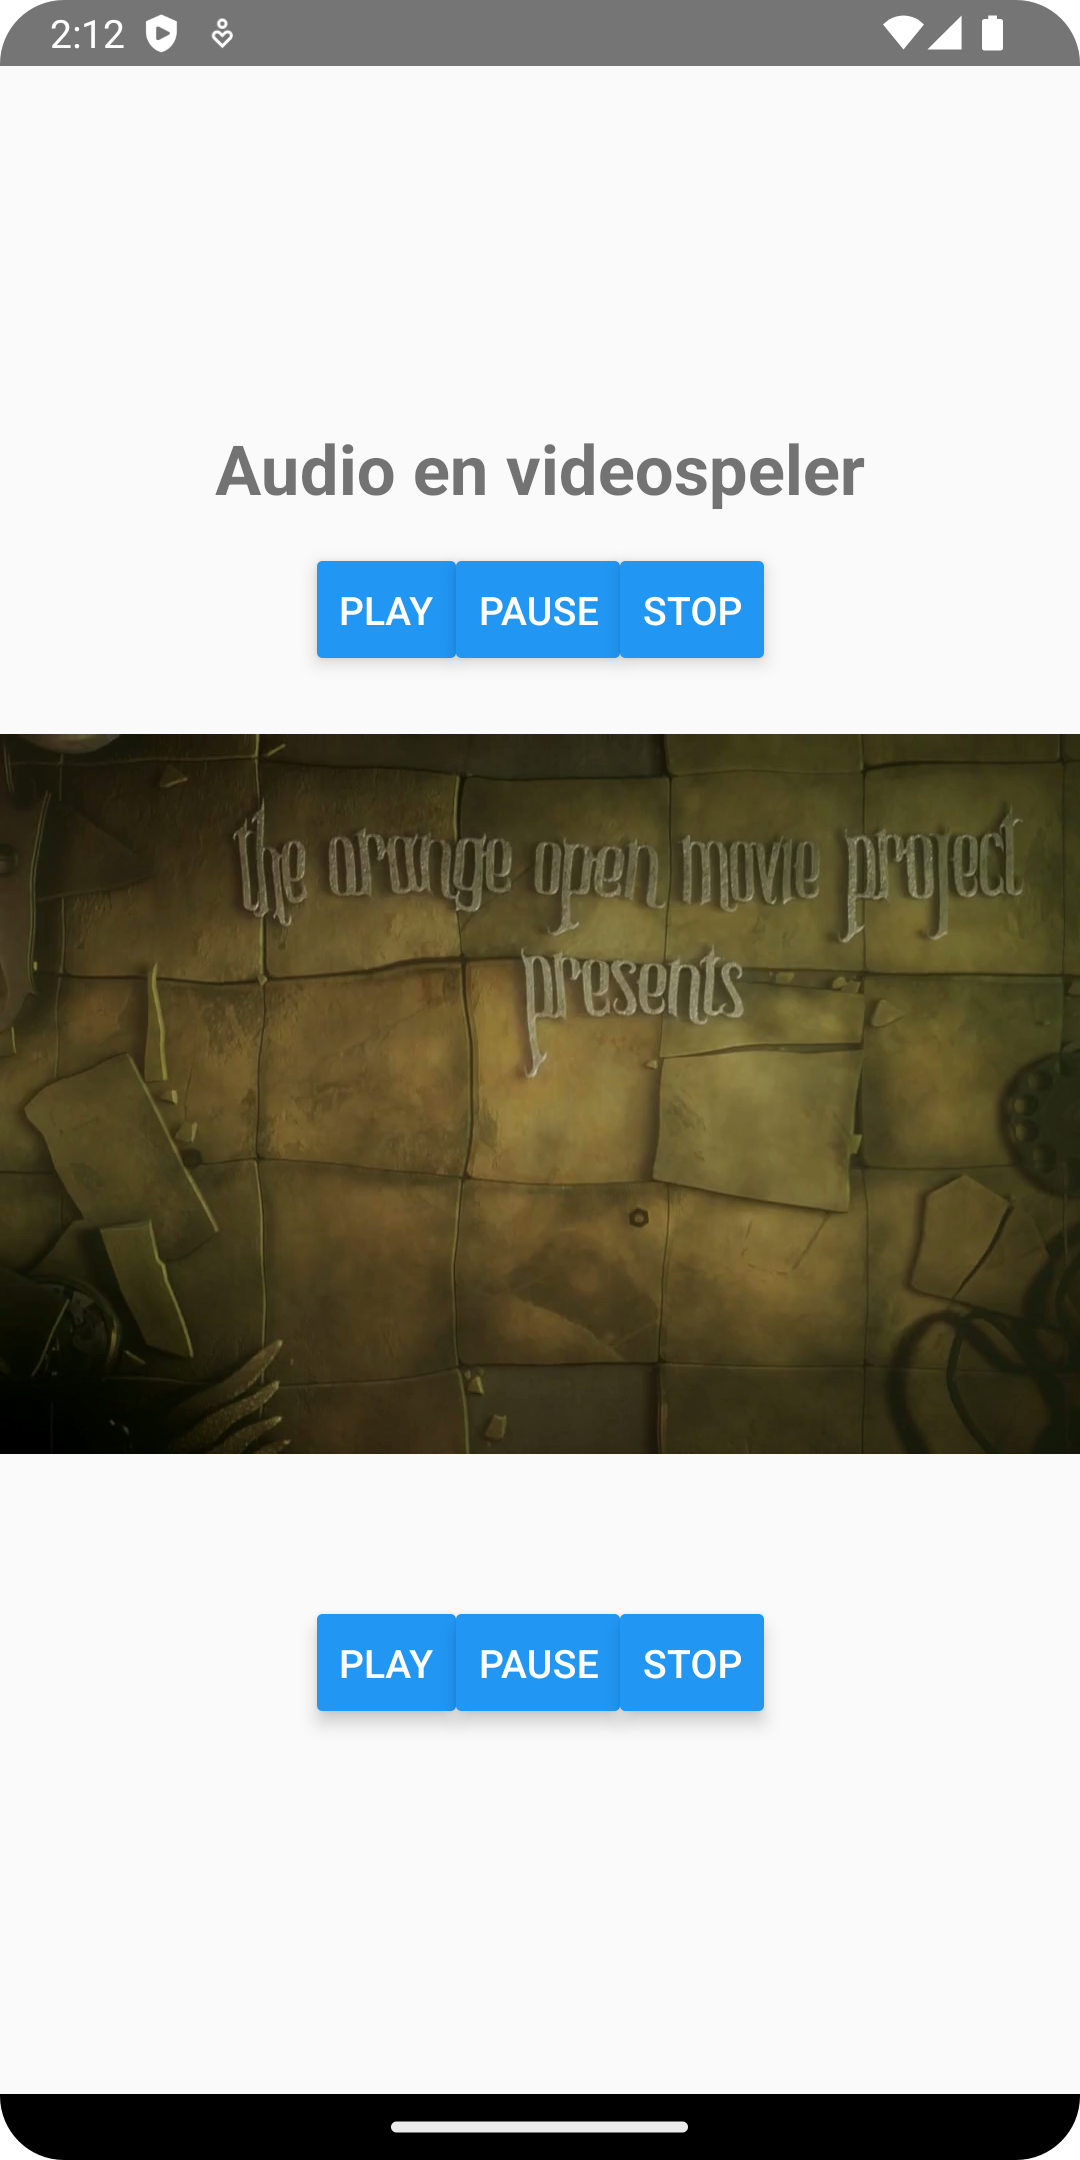
\includegraphics[height=0.4\textheight]{media_layoutcross.png}
    \caption{Layout van applicatie voor het afspelen van audio en video bij React Native.}
\end{figure}


